\chapter{Konfiguracja systemu}

\section{Plik konfiguracyjny}
Rozdział ten został poświęcony omówieniu sposobu konfiguracji systemu. Opis ten jest wstępem do szczegółowego omówienia projektu i~implementacji systemu. Konfiguracja systemu odbywa się poprzez plik typu XML, którego nazwa ustalona została przez autora na \textquote{HelloReviewConfig.xml}. Plik ten musi znajdować się folderze, z~którego zostaje uruchomiony system. Jego obecność, jak i~wszystkich składowych znaczników jest obligatoryjna do poprawnego uruchomienia i~działania systemu. Przykład konfiguracji ilustruje rysunek \ref{obr03}, który przestawia zrzut zawartości przykładowego pliku konfiguracyjnego.

\begin{figure}[!h]
\centering
    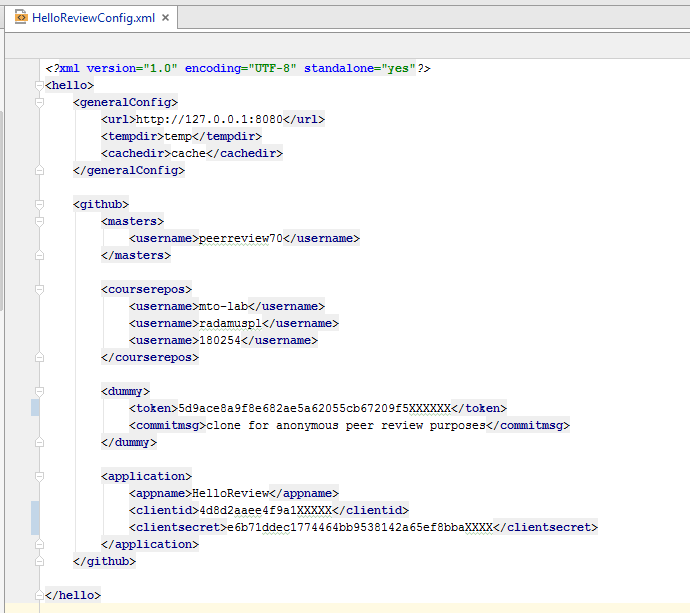
\includegraphics[width=400px]{0_3konfiguracja}
    \caption{Konfiguracja systemu - przykładowy plik}
    \label{obr03}
\end{figure}

\clearpage

Sekcja \textquote{generalConfig} zawiera zgrupowane ogólne luźno powiązane parametry ogólnego przeznaczenia:
\begin{itemize}
    \item url - adres URL do systemu, wykorzystywany jest on podczas autoryzacji przy użyciu protokołu OAuth2;
    \item tempdir - względna lub bezwzględna ścieżka do katalogu, który będzie wykorzystywany jako folder dla plików tymczasowych podczas anonimizacji prac;
    \item cachedir - względna lub bezwzględna ścieżka do katalogu, który będzie wykorzystywany jako pamięć podręczna podczas wykonywania połączeń do GitHub API.
\end{itemize}

\medskip
Sekcja \textquote{github} zawiera konfiguracje związane z~usługą GitHub.

Podsekcja \textquote{masters} zawiera listę nazw kont w~usłudze GitHub, należące do osób, które w~systemie posiadają uprawnienia prowadzących kurs.

Podsekcja \textquote{courserepos} zawiera listę nazw kont w~usłudze GitHub, które są wykorzystywane podczas kursów. Konta te wykorzystywane są jako źródło kursów. Na ich podstawie tworzona jest lista wyboru kursu podczas tworzenia nowego zlecenia przeglądu.

Podsekcja \textquote{dummy} zawiera token aplikacyjny usługi GitHub dla konta, które będzie wykorzystywane do anonimizacji prac. Na tym koncie przechowywane będą anonimowe kopie. Ponad to w~tej podsekcji ustawiony jest domyślny tekst dla akcji \textquote{commit} w~systemie kontroli wersji Git. Tekst ten zostanie użyty podczas procesu anonimizacji prac.

Podsekcja \textquote{application} definiuje dane autoryzujące aplikację w~usłudze GitHub.

\medskip
Znaczenie parametrów konfiguracji zostanie ściślej określone w~kolejnych rozdziałach, przy okazji opisu miejsc, gdzie są one wykorzystane.

\clearpage
\section{Rejestracja aplikacji w~usłudze GitHub}
Z uwagi na dużą skalę integracji z~usługą GitHub istotna część konfiguracji systemu jest związania właśnie z~tym serwisem. Autor zaleca rejestrację specjalnego konta przeznaczonego do użycia wyłączenie dla celów systemu. Jest to głównie związane z~tym, że składowane na nim będą anonimowe kopie ocenianych prac. Łatwo policzyć, że jeżeli na kurs chodzi 20 uczestników i~w danym momencie zarejestrujemy tylko jeden przegląd, gdzie każdy będzie musiał ocenić tylko jedną pracę to już jest 20 repozytoriów, które nie wyglądają profesjonalnie na koncie, i~odwracają uwagę od wartościowej zawartości. Ich ilość może być na tyle przytłaczająca, że inne treści zostaną zupełnie niezauważone.

\medskip
Rysunek nr \ref{obr04} zawiera zrzut ekranowy z~przykładem poprawnie zarejestrowanej aplikacji w~serwisie GitHub. Nazwę (\textquote{Application name}) i~opis (\textquote{Application description}) można dowolnie zmieniać. Istotne są natomiast adresy URL (\textquote{Homepage URL} i~\textquote{Authorization callback URL}). Ten pierwszy wskazuje na stronę domową, ten drugi natomiast musi wskazywać na podstronę \textquote{/callback}. To pod ten adres usługa GitHub przekieruje użytkownika po procesie logowania. Jest to jedyny poprawny adres, pod którym zostanie obsłużona informacja zwrotna.

\medskip
Ilustrowana strona zawiera także ciągi znaków \textquote{Client ID} i~\textquote{Client Secret}, które należy wprowadzić w~pliku konfiguracyjnym systemu. Istotne jest, aby ciąg \textquote{Client Secret} nie upubliczniać. Jest to ciąg związany z~mechanizmem autoryzacji \textquote{tożsamości} rejestrowanej aplikacji.

\begin{figure}[!h]
\centering
    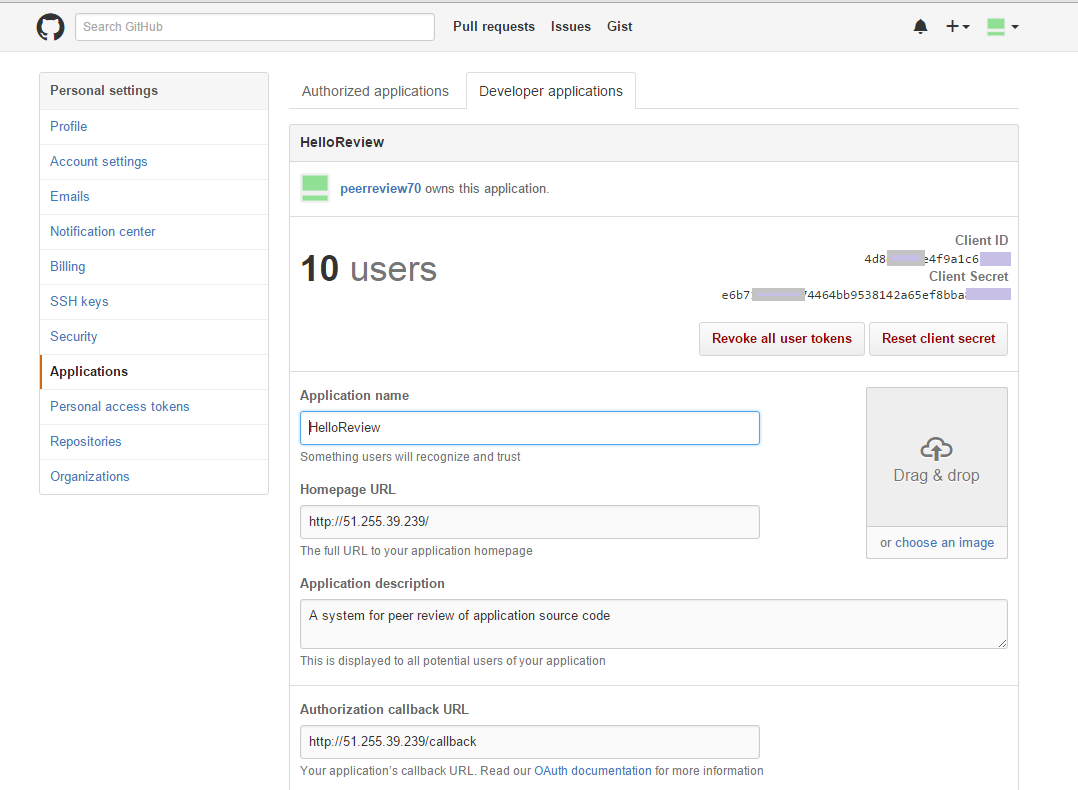
\includegraphics[width=340px]{0_4githubapp}
    \caption{Zrzut ekranowy: zarejestrowana aplikacja w~usłudze GitHub}
    \label{obr04}
\end{figure}

% ex: set tabstop=4 shiftwidth=4 softtabstop=4 noexpandtab fileformat=unix filetype=tex spelllang=pl,en spell: